\chapter{Background} \label{chap:background}

\section{Deep Learning} \label{sec:deeplearning}
\subsection{Motivations}
Deep learning has recently been highly successful in machine learning across a variety of application domains, including computer vision, natural language processing, and big data analysis, among others. For example, deep learning methods have consistently outperformed traditional methods for object recognition and detection in the ISLVRC Computer Vision Competition since 2012 \cite{ILSVRC15}. However, deep learning’s high accuracy comes at the expense of high computational and memory requirements for both the training and inference phases of deep learning. Training a deep learning model is space and computationally expensive due to millions of parameters that need to be iteratively refined over multiple time epochs. Inference is computationally expensive due to the potentially high dimensionality of the input data (e.g., a high-resolution image) and millions of computations that need to be performed on the input data.

\subsection{Definitions}
As described in \cite{Goodfellow-et-al-2016}, the modern term "deep learning" goes beyond the neuroscientific perspective engineering applications on the current breed of machine learning models. It appeals to a more general principle of learning \textit{multiple levels of composition}, which can be applied in machine learning frameworks that are not necessarily neurally inspired. Deep learning is a subset of AI and machine learning and differs in that they can automatically learn representations from data such as images, video or text, to be used for classification without introducing hand-coded rules or human domain knowledge. Their highly flexible architectures can learn directly from raw data and can increase their predictive accuracy when provided with more data.
A deep learning prediction algorithm, consists of a number of layers, as shown in Fig. \ref{fig:dnn}.

\begin{figure}
	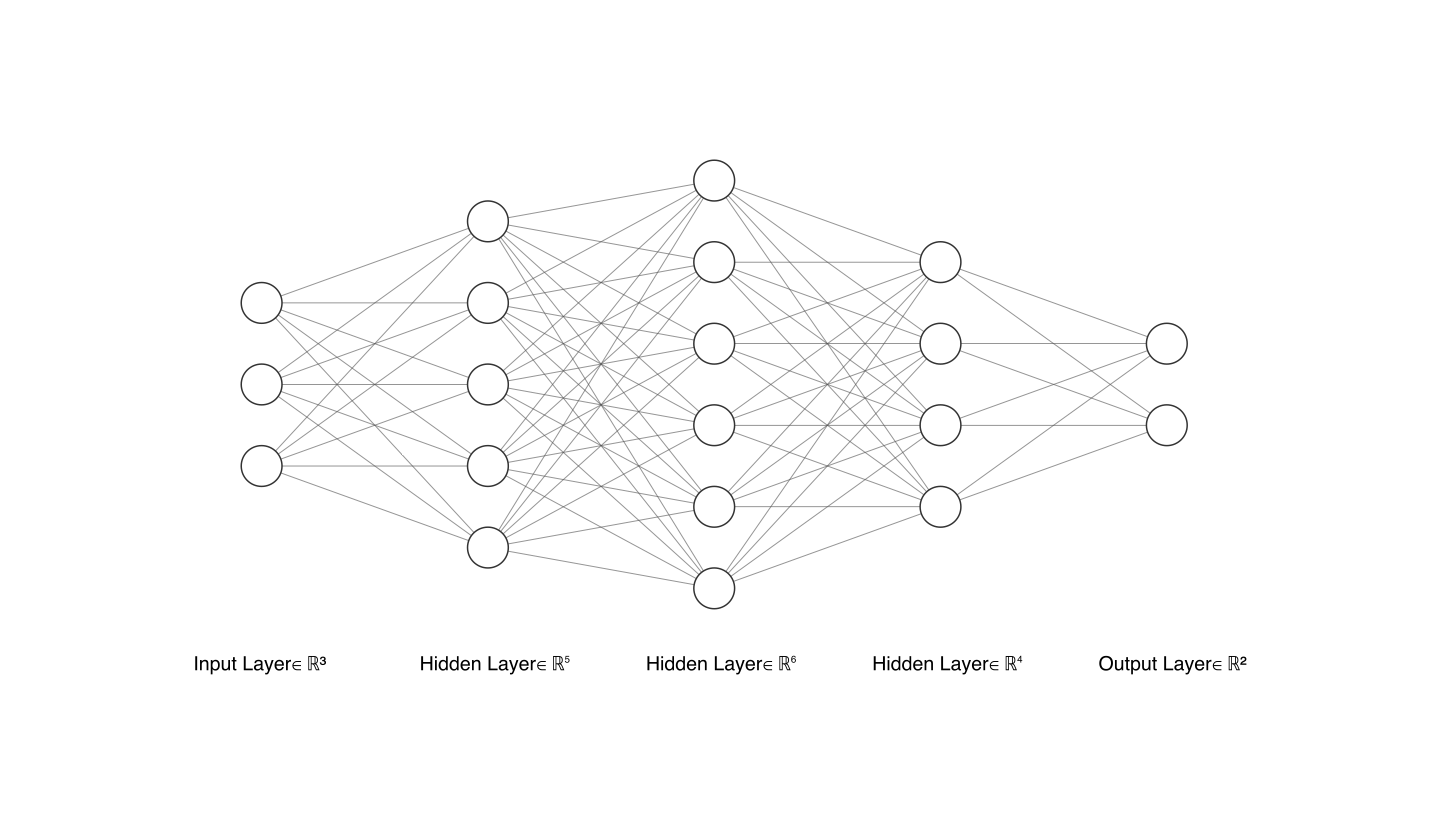
\includegraphics[width=\linewidth]{images/nn.png}
	\caption[DNN example]{DNN example with image classification}
	\label{fig:dnn}
\end{figure}

In deep learning \textit{inference}, the input data pass through the node's layers in sequence, and each layer performs matrix multiplications on the data. The output of a layer is usually the input to the subsequent layer. After data are processed by the final (fully connected) layer, the output is either a feature or a classification value. When the model contains many layers in sequence, the neural network is known as a deep neural network (DNN). When the matrix multiplications include convolutional filter operations, the model is named convolutional neural networks (CNNs), which is common for image and video processing contexts. There are also DNNs designed especially for time series prediction; these are called recurrent neural networks (RNNs), which have loops in their layer connections to keep state and enable predictions on sequential inputs.

In deep learning \textit{training}, the computation proceeds in reverse order. Given the ground-truth training labels, multiple passes are made over the layers to optimize the parameters of each layer of matrix multiplications, starting from the final layer and ending with the first layer. The algorithm used is typically stochastic gradient descent (SGD).  In each pass, a randomly small subset of N input data ("mini-batch") from the training data set, is selected and used to update the gradients in the direction that minimizes the training loss (where the training loss is defined as the difference between the predictions and the ground truth). One pass through the entire training data set is called a training epoch \cite{ruder2016overview}.

There are some considerations to take into account: the first is that there are a large number of parameters in the matrix multiplications, resulting in many computations being performed and thus the latency issues that we see on end devices. The second is that there are many choices (hyper-parameters) on how to design the DNN models (e.g., the number of parameters per layer, and the number of layers), which makes the model design more of an art than a science. Different DNN design decisions result in tradeoffs between system metrics; for example, a DNN with higher accuracy likely requires more memory to store all the model parameters and will have higher latency because of all the matrix multiplications being performed. On the other hand, a DNN model with fewer parameters will likely execute more quickly and use less computational resources and energy, but it may not have sufficient accuracy to meet the application's requirements.


\subsection{Performance Measurement}
How can we evaluate the performance of a neural network?
Deep learning can be used to perform both supervised learning and unsupervised learning. The metrics of success depend on the particular application domain where deep learning is being applied. For example, in object detection, the accuracy may be measured by the mean average precision (mAP) \cite{ILSVRC15}, which measures how well the predicted object location overlaps with the ground-truth location, averaged across multiple categories of objects. In machine translation, the accuracy can be measured by the bilingual evaluation understudy score metric \cite{10.3115/1073083.1073135}, which compares a candidate translation with several groundtruth reference translations. 
Other general system performance metrics not specific to the application include throughput, latency, and energy. These metrics are summarized in Table \ref{tab:NN-Perfomance-Metrics}.
Designing a good DNN model or selecting the right DNN model for a given application is challenging due to the large number of hyperparameter decisions.

\begin{table}[htbp]
	\centering
	\begin{tabular}{|l||c|} 
	\hline 
	 Metric & Unit	\\
	\hline
	Latency  &	s	\\
	Energy	& mW, J	\\
	Concurrent Requests Served	&	\#  \\
	Network Bandwidth	& Mbps			  \\
	Accuracy & Application Specific		\\
	\hline
	\end{tabular}
	\caption{Neural Network Perfomance Metrics\label{tab:NN-Perfomance-Metrics}}
\end{table}

Machine learning research typically focuses on accuracy metrics, and their system performance results are often reported from powerful server testbeds equipped with GPUs. For example, Huang et al. \cite{huang2016speedaccuracy} compared the speed and accuracy tradeoffs when running on a high-end gaming GPU (NVIDIA Titan X). The YOLO DNN model \cite{YOLO9000}, which is designed for real-time performance, provides timing measurements on the same server GPU.
Specifically targeting mobile devices, Lu et al. \cite{CNN-mobile} provided the measurements for a number of popular DNN models on mobile CPUs and GPUs (Nvidia TK1 and TX1). Ran et al.\cite{Ran-DNN-edge-video-analisys} further explored the accuracy-latency tradeoffs on mobile devices by measuring how reducing the dimensionality of the input size reduces the overall accuracy and latency. DNN models designed specifically for mobile devices, such as MobileNets \cite{howard2017mobilenets}, report system performance in terms of a number of multiply–add operations, which could be used to estimate latency characteristics and other metrics on different mobile hardware, based on the processing capabilities of the hardware.
Once the system performance is understood, the application developer can choose the right model. 


\subsection{Frameworks}
Several open-source software libraries are publicly available for deep learning inference and training on end devices and edge servers. Google’s TensorFlow \cite{tensorflow2015-whitepaper}, released in 2015, is an interface for expressing machine learning algorithms and an implementation for executing such algorithms on heterogeneous distributed systems. Tensorflow's computation workflow is designed as a directed graph and utilizes a placement algorithm to distribute computation tasks based on the estimated or measured execution time and communication time \cite{abadi2016tensorflow}. The placement algorithm uses a greedy approach that places a computation task on the node that is expected to complete the computation the soonest. Tensorflow can run on edge devices, such as Raspberry Pi and smartphones. TensorFlow Lite was proposed in the late 2017 \cite{tensorflowlite}, which is an optimized version of Tensorflow for mobile and embedded devices, with mobile GPU support added in early 2019. 
Tensorflow Lite only provides on-device inference abilities, not training, and achieves low latency by compressing a pre-trained DNN model.
Caffe \cite{Caffe} is another deep learning framework, originally developed by Jia, with the current version, Caffe2, maintained by Facebook. It seeks to provide an easy and straightforward way for deep learning with a focus on mobile devices, including smartphones and Raspberry Pis. PyTorch \cite{NEURIPS2019_9015} is another deep learning platform developed by Facebook, with its main goal differing from Caffe2 in which it focuses on the integration of research proto- types to production development. Actually Facebook is working on the merge of Caffe2 and PyTorch frameworks.
GPUs are an important key element in efficient DNN inference and training. NVIDIA provides GPU software libraries to make use of NVIDIA GPUs, such as CUDA \cite{CUDA} for general GPU processing and cuDNN \cite{cuDNN} which is targeted toward deep learning. While such libraries are useful for training DNN models on a desktop server, cuDNN and CUDA are not widely available on current mobile devices such as smartphones. To utilize smartphone GPUs, Android devel- opers can currently make use of Tensorflow Lite, which provides experimental GPU capabilities. To experiment with edge devices other than smartphones, researchers can turn to edge-specific development kits, such as the NVIDIA Jetson TX2 development kit for experimenting with edge computing, with NVIDIA-provided SDKs used to program the devices.



\subsection{Challenges}
Because of the required competences and effort to choose the best neural network and the best parameters that better fit the applications of our interest, there has also been much recent studies in automated machine learning, which uses artificial intelligence to choose which DNN model to run and tune the hyperparameters. 
For example, Tan et al. \cite{tan2018mnasnet} and Taylor et al. \cite{taylor2018adaptive} proposed using reinforcement learning and traditional machine learning, respectively, to choose the right hyperparameters for mobile devices, which is useful in edge scenarios.
As described in \cite{deepedgerev} many challenges remain in deploying deep learning on the edge, not only on end devices but also on the edge servers and on a combination of end devices, edge servers, and the cloud. For example parameters like latency, energy consumption and migration still the main challenges in the field of deep learning applied to the edge computing.



%%%%%%%%%%%%%%%%%%%%%%%%%%%%%%%%%%%%
\section{Edge Computing} %TODO
Today, an IoT solution has to cover a much broader scope of requirements. We see that in most cases, organizations opt for a combination of cloud and edge computing for complex IoT solutions. Cloud computing typically comes into play when organizations require storage and computing power to execute certain applications and processes, and to visualize telemetry data from anywhere. Edge computing, on the other hand, is the right choice in cases with low latency, local autonomous actions, reduced back-end traffic, and when confidential data is involved.

\subsection{Motivations}
As written in \cite{edgecomputingvision} there are at least three reasons to consider the adoption of the edge computing. The first is that putting all the computing tasks on the cloud has been proved to be an efficient way for data processing since the computing power on the cloud outclasses the capability of the things at the edge. However, compared to the fast developing data processing speed, the bandwidth of the network has come to a standstill. With the growing quantity of data generated at the edge, speed of data transportation is becoming the bottleneck for the cloud-based computing paradigm.
The second reason is that almost all kinds of electrical devices will become part of IoT, and they will play the role of data producers as well as consumers, such as air quality sensors, LED bars, streetlights and even an Internet-connected microwave oven. It is safe to infer that the number of things at the edge of the network will develop to more than billions in a few
years. Thus, raw data produced by them will be enormous, making conventional cloud computing not efficient enough to handle all these data. This means most of the data produced by IoT will never be transmitted to the cloud, instead it will be consumed at the edge of the network. Fig. \ref{fig:cloudarch} shows the conventional cloud computing structure.

\begin{figure}
	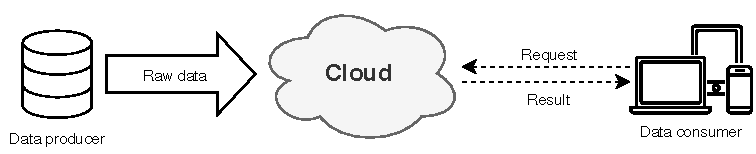
\includegraphics[width=\linewidth]{images/cloudarch}
	\caption{Cloud computing paradigm}
	\label{fig:cloudarch}
\end{figure}

However, this structure is not sufficient for IoT. First, data quantity at the edge is too large, which will lead to huge unnecessary bandwidth and computing resource usage. Second, the privacy protection requirement will pose an obstacle for cloud computing in IoT. Lastly, most of the end nodes in IoT are energy constrained things, and the wireless communication module is usually very energy hungry, so offloading some computing tasks to the edge could be more energy efficient.
Another valid consideration to take into account is that in the cloud computing paradigm, the end devices at the edge usually play as data consumer, for example, watching a YouTube video on
your smart phone. However, people are also producing data nowadays from their mobile devices. The change from data consumer to data producer/consumer requires more function placement at the edge.


\subsection{Definitions}
Edge computing refers to the enabling technologies allowing computation to be performed at the edge of the network, on downstream data on behalf of cloud services and upstream data on behalf of IoT services. The rationale of edge computing is that computing should happen at the proximity of data sources. From a certain point of view, edge computing could interchangeable with fog computing \cite{openfog}, but edge computing focus more toward the things side, while the first focus more on the infrastructure side. Fig. \ref{fig:edgearch} illustrates the two-way computing streams in edge computing. In the edge computing paradigm, the things not only are data consumers, but also play as data producers. At the edge, the things can not only request service and content from the cloud but also perform the computing tasks from the cloud. Edge can perform computing offloading, data storage, caching and processing, as well as distribute request and delivery service from cloud to user. With those jobs in the network, the edge itself needs to be well designed to meet the requirement efficiently in service such as reliability, security, and privacy protection.

\begin{figure}
	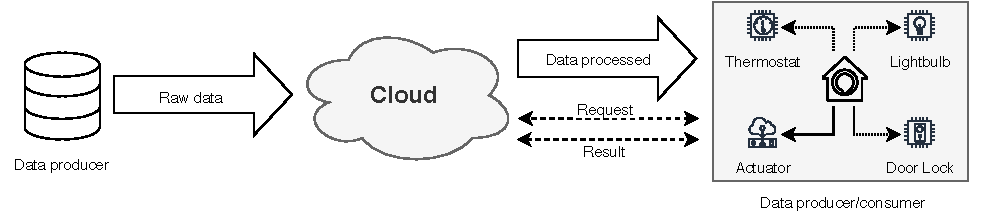
\includegraphics[width=\linewidth]{images/edgearch}
	\caption{Edge computing paradigm}
	\label{fig:edgearch}
\end{figure}


\subsection{Performance metrics}
In edge computing, we have multiple layers with different computation capability. Workload allocation becomes a big
issue. We need to decide which layer to handle the workload or how many tasks to assign at each part. There are multiple allocation strategies to complete a workload, for instances,
evenly distribute the workload on each layer or complete as much as possible on each layer To choose an optimal allocation strategy, there several optimization parameter to consider. These metrics are very similar to those described in \ref{sec:deeplearning}, including latency, bandwidth and energy. How to measure these performance is strongly dependent by the environment, resources and application case.


\subsection{Challenges}
In cloud computing, users program their code and deploy them on the cloud. Usually, the program is written in one programming language and compiled for a certain target platform, since the program only runs in the cloud. However, in the edge computing, computation is offloaded from the cloud, and the edge nodes are most likely heterogeneous platforms. In this case, the runtime of these nodes differ from each other, and the programmer faces huge difficulties to write an application that may be deployed in the edge computing paradigm.
Another important challenge is related to the \textit{naming}. In edge computing, one important assumption is that the number of things is tremendously large. At the top of the edge nodes, there are a lot of applications running, and each application has its own structure about how the service is provided. Similar to all computer systems, the naming scheme in edge computing is very important for development, addressing, things identification, and data communication. However, an efficient naming mechanism for the edge computing paradigm has not been built and standardized yet. Edge practitioners usually needs to learn various communication and network protocols in order to communicate with the heterogeneous things in their system.
In terms of \textit{service management} at the edge of the network, there are four fundamental features that should be supported to guarantee a reliable system, including differentiation, extensibility, isolation, and reliability.  
To protect the data \textit{security} and usage \textit{privacy} at the edge of the network, several challenges remain open. First is the awareness of privacy and security to the community: ip camera, health monitor, or even some WiFi enabled toys could easily be connected by others if not protected properly. Second is the ownership of the data collected from things at edge. Just as what happened with mobile applications, the data of end user collected by things will be stored and analyzed at the service provider side. Third is the missing of efficient tools to protect data privacy and security at the edge of the network. The highly dynamic environment at the edge of the network also makes the network become vulnerable or unprotected and more tools are still missing to handle diverse data attributes for edge computing.


%%%%%%%%%%%%%%%%%%%%%%%%%%%%%%%%%%%%
\section{Robotics Tools and Platforms} \label{sec:Robotics-Tools-and-Platforms}
This section will cite and recap the main robotics platforms discovered and explored during the development of this thesis.

\subsection{ROS}
The Robot Operating System (ROS) \cite{ROS}, is a open-source framework based on the component-based software engineering paradigm that provides the middleware for inter-process communication. Initially developed by the Stanford  Artificial Intelligence Laboratory its development continued at Willow Garage, a robotics research institute, and now it's maintained and improved under the action of the ORSF foundation \cite{ROS}. As a meta-operating system, ROS offers features such as hardware abstraction, low-level device control, implementation of commonly used functionalities, message communication between processes and package management. It uses an asynchronous publish/subscribing mechanism made possible by message standardisation and encapsulation that make the external interface of every node as general as possible, allowing quick nodes exchange and, thus, great architectural flexibility. Each independent block, called \textit{node}, executes a particular task of a process and can communicates with other nodes through \textit{topics}. This allows to create complex architectures by aggregating many simpler entities and simplifies the use of different tasks  or different methods for the same task. Additionally to the message-passing system, the core ROS component, called \textit{roscore}, maintains a global execution time for the nodes to achieve synchronisation. Each node executes separately with its own internal clock driven by the set execution rate. At every message sent/received, containing the internal time information, the core component updates the global time by following the execution status provided by these messages.
For more clarity about how ROS communication works an example is provided in figure \ref{fig:ros-nodes-topics}. When a publishing node will announce to the master that it is publishing over a topic and the subscribing node will say to the master that it want to listen to a topic. Then if the publisher
and the subscriber are on the same topic, the master will transfer data in order for the two other node to communicate directly via TCP/IP or UDP.

\begin{figure}[htbp]
	\centering
	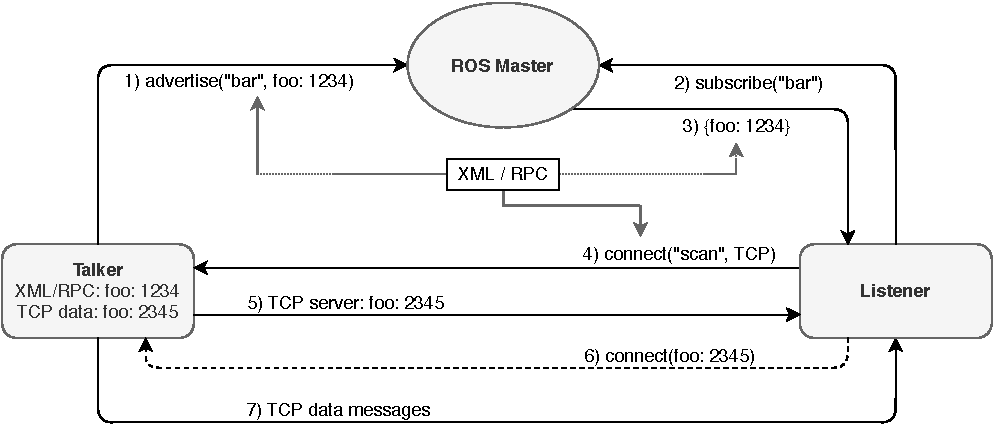
\includegraphics[width=0.90\textwidth]{images/ROSexample2.pdf}
	\caption{Example of nodes and topic communication}
	\label{fig:ros-nodes-topics}
\end{figure}

The reason to choose ROS for the development of robotics applications resides mainly in its high modularity. Furthermore it is a well known standard in the scientific community of the robotics researches and developers.




\subsection{NVIDIA Isaac SDK}
The Isaac SDK is the main software toolkit provided by NVIDIA and allows developers to brought new opportunities for developing robotics solutions as well as researching topics in this field. As described in \cite{ISAAC} it's comprised of the following:
\begin{itemize}
	\item Isaac Robot Engine: A framework which allows you to easily write modular applications and deploy them on your robots.
	\item Isaac GEMs: A collection of robotics algorithms from planning to perception, most of them GPU-accelerated.
	\item Applications: Various example applications from basic samples which show specific features to applications that facilitate complicated robotics use cases.
	\item Isaac Sim for Navigation: A powerful virtual robotics laboratory and a high-fidelity 3D world simulator that accelerates research, design, and development by reducing cost and risk.
\end{itemize}

The main reasons we would consider to use this platform reside in its high modularity and high performance solutions that it is able to offer on NVIDIA Jetson platforms.
Others important reasons to adopt this solution are related the \textbf{C API} that allows the communication with Isaac apps from languages other than C++, and the \textbf{ROS bridge} that offers the capability to interact with ROS nodes applications.

%TODO put an images that shows the Isaac architecture

\subsection{CoppeliaSim}
From the creators of V-Rep \cite{VREP}, CoppeliaSim \cite{coppeliaSim} seems to be the definitive solution for development of robotics applications.
The robot simulator CoppeliaSim, with integrated development environment, is based on a distributed control architecture: each object/model can be individually controlled via an embedded script, a plugin, ROS nodes, BlueZero nodes, remote API clients, or a custom solution. This makes CoppeliaSim very versatile and ideal for multi-robot applications. Controllers can be written in C/C++, Python, Java, Lua, Matlab, Octave or Urbi.
CoppeliaSim can be used as a stand-alone application or can easily be embedded into a main client application: its small footprint and elaborate API makes CoppeliaSim an ideal candidate to embed into higher-level applications. An integrated Lua script interpreter makes CoppeliaSim an extremely versatile application, leaving the freedom to the user to combine the low/high-level functionalities to obtain new high-level functionalities.




%%%%%%%%%%%%%%%%%%%%%%%%%%%%%%%%%%%%
\section{Docker} %TODO




%%%%%%%%%%%%%%%%%%%%%%%%%%%%%%%%%%%%
\section{Kubernetes} \label{kubernetesbackground} %TODO



%%%%%%%%%%%%%%%%%%%%%%%%%%%%%%%%%%%%
\section{Kubeedge} \label{kubeedgebackground} %TODO
\clearpage
\thispagestyle{empty}